\section{Anwendung \label{kra:section:anwendung}}
\rhead{Anwendung}

Die Matrix-Riccati Differentialgleichung findet unter anderem Anwendung in der Regelungstechnik beim RQ- und RQG-Regler oder aber auch beim Kalman-Filter.
Im folgenden Abschnitt möchten wir uns an einem Beispiel anschauen wie wir mit Hilfe der Matrix-Riccati-Differentialgleichung (\ref{kra:equation:matrixriccati}) ein Feder-Masse-System untersuchen können \cite{kra:riccati}.

\subsection{Feder-Masse-System}
\label{kra:subsection:feder-masse-system}
Die einfachste Form eines Feder-Masse-Systems ist dargestellt in Abbildung~\ref{kra:fig:simple_mass_spring}.
Es besteht aus einer reibungsfrei gelagerten Masse $m$, welche an eine Feder mit der Federkonstante $k$ gekoppelt ist.
Die im System wirkenden Kräfte teilen sich auf in die auf dem hookeschen Gesetz basierenden Rückstellkraft $F_R = k \Delta_x$ und der auf dem Aktionsprinzip basierenden Kraft $F_a = am = \ddot{x} m$.
Das Kräftegleichgewicht fordert $F_R = F_a$ woraus folgt, dass

\begin{equation*}
    k \Delta_x = \ddot{x} m \Leftrightarrow \ddot{x} = \frac{k \Delta_x}{m}.
\end{equation*}
Die Funktion die diese Differentialgleichung löst, ist die harmonische Schwingung
\begin{equation}
    x(t) = A \cos(\omega_0 t + \varphi), \quad \omega_0 = \sqrt{\frac{k}{m}}.
\end{equation}
\begin{figure}
    \centering
    % move image to standalone because the physics package is
    % incompatible with underbrace
    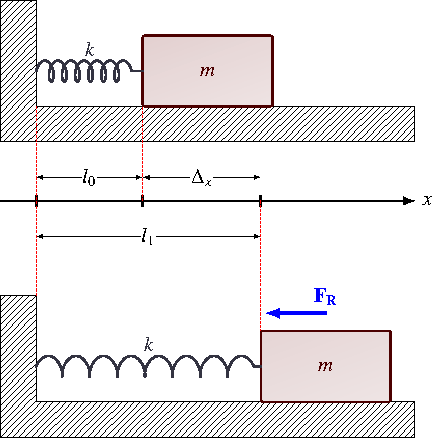
\includegraphics{papers/kra/images/simple.pdf}
    %% create tikz drawing of a simple mass spring system

\tikzstyle{hmline}=[{Latex[length=3.3,width=2.2]}-{Latex[length=3.3,width=2.2]},line width=0.3]
\tikzstyle{vmline}=[red, dashed,line width=0.4,dash pattern=on 1pt off 1pt]
\tikzstyle{ground}=[pattern=north east lines]
\tikzstyle{mass}=[line width=0.6,red!30!black,fill=red!40!black!10,rounded corners=1,top color=red!40!black!20,bottom color=red!40!black!10,shading angle=20]
\tikzstyle{spring}=[line width=0.8,blue!7!black!80,snake=coil,segment amplitude=5,line cap=round]

\begin{tikzpicture}[scale=2]
    \newcommand{\ticks}[2]
    {
        % arguments: x, y coordinates
        \draw[thick] (#1, #2 - 0.1 / 2) --++ (0, 0.1);
    }

    \tikzmath{
        \hWall = 1.2;
        \wWall = 0.3;
        \lWall = 3.5;
        \hMass = 0.6;
        \wMass = 1.1;
        \xMass1 = 1.2;
        \xMass2 = 2.2;
        \xAxisYpos = 0;
        \originX1 = 0;
        \originY1 = 0.5;
        \originX2 = 0;
        \originY2 = -2;
        \springscale=7;
    }

    % create x axis
    \draw[->,thick] (0,\xAxisYpos) --+ (\lWall, 0) node[right]{$x$};

    % create ticks on x axis
    \ticks{\wWall}{\xAxisYpos}
    \ticks{\xMass1}{\xAxisYpos}
    \ticks{\xMass2}{\xAxisYpos}

    % create underground
    \draw[ground] (\originX1, \originY1) ++ (0, 0) --+(\lWall,0) --+(\lWall, \wWall) --+(\wWall, \wWall) --+(\wWall, \hWall) --+(0, \hWall) -- cycle;
    \draw[ground] (\originX2, \originY2) ++ (0, 0) --+(\lWall,0) --+(\lWall, \wWall) --+(\wWall, \wWall) --+(\wWall, \hWall) --+(0, \hWall) -- cycle;

    % create masses
    \draw[mass] (\originX1, \originY1) ++ (\xMass1, \wWall) rectangle ++ (\wMass,\hMass) node[midway] {$m$};
    \draw[mass] (\originX2, \originY2) ++ (\xMass2, \wWall) rectangle ++ (\wMass,\hMass) node[midway] {$m$};

    % create springs
    \draw[spring, segment length=(\xMass1 - \wWall) * \springscale] (\originX1, \originY1) ++
    (\wWall, \wWall + \hMass / 2) --++ (\xMass1 - \wWall, 0) node[midway,above=0.2] {$k$};
    \draw[spring, segment length=(\xMass2 - \wWall) * \springscale] (\originX2, \originY2) ++
    (\wWall, \wWall + \hMass / 2) --++ (\xMass2 - \wWall, 0) node[midway,above=0.2] {$k$};

    % create vertical measurement line 
    \draw[vmline] (\xMass1, \xAxisYpos) --+(0, \originY1 + \wWall);
    \draw[vmline] (\xMass2, \xAxisYpos) --+(0, \originY2 + \hMass+\wWall);
    \draw[vmline] (\wWall, \originY1+\wWall) --(\wWall, \originY2 + \hWall);

    % create horizontal measurement line
    \draw[hmline] (\wWall, \xAxisYpos + 0.2) -- (\xMass1, \xAxisYpos + 0.2) node[midway,fill=white,inner sep=0] {$\ell_0$};
    \draw[hmline] (\xMass1, \xAxisYpos + 0.2) -- (\xMass2, \xAxisYpos + 0.2) node[midway,fill=white,inner sep=0] {$\Delta_{x}$};
    \draw[hmline] (\wWall, \xAxisYpos - 0.3) -- (\xMass2, \xAxisYpos - 0.3) node[midway,fill=white,inner sep=0] {$\ell_{1}$};

    %  create force arrow
    \draw[->,blue, very thick,line cap=round] (\xMass2 + \wMass / 2, \originY2 + \wWall + \hMass + 0.15) node[above] {$\vb{F_{R}}$} --+ (-0.5, 0);
\end{tikzpicture}
    \caption{Einfaches Feder-Masse-System.}
    \label{kra:fig:simple_mass_spring}
\end{figure}
\begin{figure}
    \centering
    % create tikz drawing of a multi mass multi spring system

\tikzstyle{vmline}=[red, dashed,line width=0.4,dash pattern=on 1pt off 1pt]
\tikzstyle{ground}=[pattern=north east lines]
\tikzstyle{mass}=[line width=0.6,red!30!black,fill=red!40!black!10,rounded corners=1,top color=red!40!black!20,bottom color=red!40!black!10,shading angle=20]
\tikzstyle{spring}=[line width=0.8,blue!7!black!80,snake=coil,segment amplitude=5,line cap=round]

\begin{tikzpicture}[scale=2]
    \newcommand{\ticks}[3]
    {
        % x, y coordinates
        \draw[thick] (#1, #2 - 0.1 / 2) --++ (0, 0.1) node[scale=0.8,below=0.2] {#3};
    }
    \tikzmath{
        \hWall = 1.2;
        \wWall = 0.3;
        \lWall = 5;
        \hMass = 0.6;
        \wMass = 1.1;
        \xMass1 = 1.0;
        \xMass2 = 3.0;
        \xAxisYpos = 0;
        \originX1 = 0;
        \originY1 = 0.5;
        \springscale=7;
    }

    % create axis
    \draw[->,thick] (0,\xAxisYpos) --+ (\xMass2 + \wMass, 0) node[right]{$q$};
    % create ticks on x / q axis
    \ticks{\xMass1}{\xAxisYpos}{$q_{1}$}
    \ticks{\xMass2}{\xAxisYpos}{$q_{2}$}

    % create non-moving backgrounds
    \draw[ground] (\originX1, \originY1) ++ (0, 0) --+(\lWall,0) --+(\lWall, \hWall)
    --+ (\lWall - \wWall, \hWall) --+(\lWall - \wWall, \wWall) --+ (\wWall, \wWall)  --+(\wWall, \hWall) --+(0, \hWall) -- cycle;

    % create masses
    \draw[mass] (\originX1, \originY1) ++ (\xMass1, \wWall) rectangle ++ (\wMass,\hMass) node[midway] {$m_{1}$};
    \draw[mass] (\originX1, \originY1) ++ (\xMass2, \wWall) rectangle ++ (\wMass,\hMass) node[midway] {$m_{2}$};

    % create springs
    \draw[spring, segment length=(\xMass1 - \wWall) * \springscale] (\originX1, \originY1) ++
    (\wWall, \wWall + \hMass / 2) --++ (\xMass1 - \wWall, 0) node[midway,above=0.2] {$k_1$};
    \draw[spring, segment length=(\xMass1 - \wWall) * \springscale] (\originX1, \originY1) ++
    (\xMass1 + \wMass, \wWall + \hMass / 2) --++ (\xMass2 - \xMass1 - \wMass, 0) node[midway,above=0.2] {$k_c$};
    \draw[spring, segment length=(\xMass1 - \wWall) * \springscale] (\originX1, \originY1) ++
    (\xMass2 + \wMass, \wWall + \hMass / 2) --++ (\lWall - \xMass2 - \wMass - \wWall, 0) node[midway,above=0.2] {$k_2$};

    % create vertical measurement line 
    \draw[vmline] (\xMass1, \xAxisYpos) --+(0, \originY1 + \wWall);
    \draw[vmline] (\xMass2, \xAxisYpos) --+(0, \originY1 + \wWall);

\end{tikzpicture}

    \caption{Feder-Masse-System mit zwei Massen und drei Federn.}
    \label{kra:fig:multi_mass_spring}
\end{figure}

\subsection{Hamilton-Funktion}
\label{kra:subsection:hamilton-funktion}
Die Bewegung der Masse $m$ kann mit Hilfe der hamiltonschen Mechanik im Phasenraum untersucht werden.
Die hamiltonschen Gleichungen verwenden dafür die verallgemeinerten Ortskoordinaten
$q = (q_{1}, q_{2}, ..., q_{n})$ und die verallgemeinerten Impulskoordinaten $p = (p_{1}, p_{2}, ..., p_{n})$, wobei der Impuls definiert ist als $p_k = m_k \cdot v_k$.
Liegen keine zeitabhängigen Zwangsbedingungen vor, so entspricht die Hamilton-Funktion der Gesamtenergie des Systems \cite{kra:hamilton}.
Im Falle des einfachen Feder-Masse-Systems, Abbildung \ref{kra:fig:simple_mass_spring}, setzt sich die Hamilton-Funktion aus kinetischer und potentieller Energie zusammen.
\begin{equation}
    \label{kra:equation:harmonischer_oszillator}
    \begin{split}
        H(q, p) &= T(p) + V(q) = E \\
        &= \underbrace{\frac{p^2}{2m}}_{\displaystyle{E_{kin}}} + \underbrace{\frac{k q^2}{2}}_{\displaystyle{E_{pot}}}
    \end{split}
\end{equation}
Die Hamiltonschen Bewegungsgleichungen liefern \cite{kra:kanonischegleichungen}
\begin{equation}
    \label{kra:equation:bewegungsgleichung}
    \dot{q_{k}} = \frac{\partial H}{\partial p_k}
    \qquad
    \dot{p_{k}} = -\frac{\partial H}{\partial q_k},
\end{equation}
daraus folgt
\[
    \dot{q} = \frac{p}{m}
    \qquad
    \dot{p} = -kq.
\]
In Matrixschreibweise erhalten wir also
\[
    \begin{pmatrix}
        \dot{q} \\
        \dot{p}
    \end{pmatrix}
    =
    \begin{pmatrix}
        0  & \frac{1}{m} \\
        -k & 0
    \end{pmatrix}
    \begin{pmatrix}
        q \\
        p
    \end{pmatrix}
    .
\]
Für das erweiterte Federmassesystem, Abbildung \ref{kra:fig:multi_mass_spring}, können wir analog vorgehen.
Die kinetische Energie setzt sich nun aus den kinetischen Energien der einzelnen Massen $m_1$ und $m_2$ zusammen.
Die potentielle Energie erhalten wir aus der Summe der kinetischen Energien der einzelnen Federn mit den Federkonstanten $k_1$, $k_c$ und $k_2$.
\begin{align*}
    \begin{split}
        T   &= T_1 + T_2 \\
        &= \frac{p_1^2}{2m_1} + \frac{p_2^2}{2m_2}
    \end{split}
    \\
    \begin{split}
        V   &= V_1 + V_c + V_2 \\
        &= \frac{k_1 q_1^2}{2} + \frac{k_c (q_2 - q_1)^2}{2} + \frac{k_2 q_2^2}{2}.
    \end{split}
\end{align*}
Die Hamilton-Funktion ist also
\begin{align*}
    \begin{split}
        H   &= T + V \\
        &= \frac{p_1^2}{2m_1} + \frac{p_2^2}{2m_2} + \frac{k_1 q_1^2}{2} + \frac{k_c (q_2 - q_1)^2}{2} + \frac{k_2 q_2^2}{2}
    \end{split}
\end{align*}
Die Bewegungsgleichungen \eqref{kra:equation:bewegungsgleichung} liefern
\begin{align*}
    \frac{\partial H}{\partial p_k}  & = \dot{q_k}
    \Rightarrow
    \left\{
    \begin{alignedat}{2}
        \dot{q_1}   &= \frac{2p_1}{2m_1}    &&= \frac{p_1}{m_1}\\
        \dot{q_2}   &= \frac{2p_2}{2m_2}    &&= \frac{p_2}{m_2}
    \end{alignedat}
    \right.
    \\
    -\frac{\partial H}{\partial q_k} & = \dot{p_k}
    \Rightarrow
    \left\{
    \begin{alignedat}{2}
        \dot{p_1}   &= -(\frac{2k_1q_1}{2} - \frac{2k_c(q_2-q_1)}{2})  &&= -q_1(k_1+k_c) + q_2k_c \\
        \dot{p_1}   &= -(\frac{2k_c(q_2-q_1)}{2} - \frac{2k_2q_2}{2})  &&= q_1k_c - (k_c + k_2).
    \end{alignedat}
    \right.
\end{align*}
In Matrixschreibweise erhalten wir
\begin{equation}
    \label{kra:equation:hamilton-multispringmass}
    \begin{pmatrix}
        \dot{q_1} \\
        \dot{q_2} \\
        \dot{p_1} \\
        \dot{p_2} \\
    \end{pmatrix}
    =
    \begin{pmatrix}
        0            & 0            & \frac{1}{2m_1} & 0              \\
        0            & 0            & 0              & \frac{1}{2m_2} \\
        -(k_1 + k_c) & k_c          & 0              & 0              \\
        k_c          & -(k_c + k_2) & 0              & 0              \\
    \end{pmatrix}
    \begin{pmatrix}
        q_1 \\
        q_2 \\
        p_1 \\
        p_2 \\
    \end{pmatrix}
    \Leftrightarrow
    \dt
    \begin{pmatrix}
        Q \\
        P \\
    \end{pmatrix}
    =
    \underbrace{
        \begin{pmatrix}
            0 & M \\
            K & 0
        \end{pmatrix}
    }_{G}
    \begin{pmatrix}
        Q \\
        P \\
    \end{pmatrix}.
\end{equation}

\subsection{Phasenraum}
\subsubsection{Motivation}
Die Beschreibung eines klassischen physikalischen Systems führt in der Newtonschen-Mechanik, wie wir in \ref{kra:subsection:feder-masse-system} gesehen haben, auf eine Differentialgleichung 2. Ordung der Dimension $n$.
Zur Betrachung des Systems verwenden wir dabei den Konfigurationsraum, ein Raum $\mathbb{R}^n$, bei dem ein einziger Punkt die Position aller $n$ Teilchen festlegt.
Der Nachteil des Konfigurationsraums ist dabei, dass dieser nur die Positionen der Teilchen widerspiegelt.
Um den Zustand eines Systems vollständig zu beschreiben, muss man aber nicht nur wissen wo sich die Teilchen zu einem bestimmten Zeitpunkt befinden, sondern auch wie sie sich bewegen.

Im Gegensatz dazu führt die Beschreibung des Systems mit Hilfe der Hamilton-Mechanik \ref{kra:subsection:hamilton-funktion}, auf eine Differentialgleichung 1. Ordnung der Dimension $2n$.
Die Betrachtung erfolgt im einem Raum $\mathbb{R}^{2n}$, bei dem ein einzelner Punkt den Bewegungszustand vollständig beschreibt, dem sogennanten Phasenraum.
Die Phasenraumdarstellung eignet sich somit sehr gut für die systematische Untersuchung der Feder-Masse-Systeme.

\subsubsection{Harmonischer Oszillator}
Die Hamiltonfunktion des harmonischen Oszillators \eqref{kra:equation:harmonischer_oszillator} führt auf eine Lösung der Form
\begin{equation*}
    q(t) = A \cos(\omega_0 T + \Phi), \quad p(t) = -m \omega_0 A \sin(\omega_0 t + \Phi),
\end{equation*}
die Phasenraumtrajektorien bilden also Ellipsen mit Zentrum $q=0, p=0$ und Halbachsen $A$ und $m \omega A$.
Abbildung~\ref{kra:fig:phasenraum} zeigt Phasenraumtrajektorien mit den Energien $E_{x \in \{A, B, C, D\}}$ und verschiedenen Werten von $\omega$.
\begin{figure}
    \centering
    \colorlet{mypurple}{red!50!blue!90!black!80}

% style to create arrows
\tikzset{
    traj/.style 2 args={thick, postaction={decorate},decoration={markings,
                    mark=at position #1 with {\arrow{<}},
                    mark=at position #2 with {\arrow{<}}}
        }
}

\begin{tikzpicture}[scale=0.6]
    % p(t=0) = 0, q(t=0) = A, max(p) = mwA
    \tikzmath{
        \axh = 5.2;
        \axw1 = 4.2;
        \axw2 = 4.8;
        \d1 = 0.9;
        \a0 = 1;
        \b0 = 2;
        \a1 = \a0 + \d1;
        \b1 = \b0 + \d1;
        \a2 = \a1 + \d1;
        \b2 = \b1 + \d1;
        \a3 = \a2 + \d1;
        \b3 = \b2 + \d1;
        \d2 = 0.75;
        \aa0 = 2;
        \bb0 = 1;
        \aa1 = \aa0 + \d2;
        \bb1 = \bb0 + \d2;
        \aa2 = \aa1 + \d2;
        \bb2 = \bb1 + \d2;
        \aa3 = \aa2 + \d2;
        \bb3 = \bb2 + \d2;
    }

    \draw[->,thick] (-\axw1,0) -- (\axw1,0) node[right] {$q$};
    \draw[->,thick] (0,-\axh) -- (0,\axh) node[above] {$p$};

    \draw[traj={0.375}{0.875},darkgreen] ellipse (\a0 and \b0);
    \draw[traj={0.375}{0.875},blue] ellipse (\a1 and \b1);
    \draw[traj={0.375}{0.875},cyan] ellipse (\a2 and \b2);
    \draw[traj={0.375}{0.875},mypurple] ellipse (\a3 and \b3);

    \node[right,darkgreen] at (45:{\a0} and {\b0}) {$E_A$};
    \node[right, blue] at (45:{\a1} and {\b1}) {$E_B$};
    \node[right, cyan] at (45:{\a2} and {\b2}) {$E_C$};
    \node[right, mypurple] at (45:{\a3} and {\b3}) {$E_D$};
    \node[above left] at (110:\b3 + 0.1) {grosses $\omega$};

    \begin{scope}[xshift=12cm]
        \draw[->,thick] (-\axw2,0) -- (\axw2,0) node[right] {$q$};
        \draw[->,thick] (0,-\axh) -- (0,\axh) node[above] {$p$};

        \draw[traj={0.375}{0.875},darkgreen] ellipse (\aa0 and \bb0);
        \draw[traj={0.375}{0.875},blue] ellipse (\aa1 and \bb1);
        \draw[traj={0.375}{0.875},cyan] ellipse (\aa2 and \bb2);
        \draw[traj={0.375}{0.875},mypurple] ellipse (\aa3 and \bb3);

        \node[above, darkgreen] at (45:{\aa0} and {\bb0}) {$E_A$};
        \node[above, blue] at (45:{\aa1} and {\bb1}) {$E_B$};
        \node[above, cyan] at (45:{\aa2} and {\bb2}) {$E_C$};
        \node[above, mypurple] at (45:{\aa3} and {\bb3}) {$E_D$};

        \node[above left] at (110:\b3 + 0.1) {kleines $\omega$};
    \end{scope}
\end{tikzpicture}
    \caption{Phasenraumdarstellung des einfachen Feder-Masse-Systems.}
    \label{kra:fig:phasenraum}
\end{figure}

\subsubsection{Erweitertes Feder-Masse-System}
Die Lösung der Gleichung \eqref{kra:equation:hamilton-multispringmass} beschreibt sowohl die zeitliche Entwicklung der Position als auch der Impulse.
Um das System im Phasenraum zu untersuchen, reicht uns aber auch die zeitliche Entwicklung des Phasenwinkels $U(t) = P(t)Q^{-1}(t)$.
Nach Satz~\ref{kra:satz:riccati-matrix-dgl} erhalten wir für die Ableitung von $U$
\begin{equation}
    \begin{split}
        \dt U   &= K  + 0U(t) - U(t)0 - U(t)MU(t) \\
        &= K + U(t)MU(t),
    \end{split}
\end{equation}
eine Riccati-Matrix-Differentialgleichung.

Im Folgenden betrachten wir uns den Fall: Anfangsbedingungen $Q(t=0)=I$ und $P(t=0)=0$.
Die Berechnung der aktuellen Positionen aus den Anfangsbedingungen ermöglicht die Matrix $Q$.
Mit Hilfe von $Q^{-1}$ können wir dann von den aktuellen Auslenkungen zurück auf Auslenkungen zur Zeit $t=0$ rechnen.
Mit $P(t)$ erhalten wir danach die zugehörige Geschwindigkeit.
Die Matrix $U(t)$ beschreibt also, wie man die aktuellen Impulse aus den Positionen berechnen kann, indem man aus der aktuellen Auslenkungsverteilung
die Anfangsauslenkungen zur Zeit $t=0$ und daraus die aktuelle Impulsverteilung berechnet.
Die Matrix-Riccati-Differentialgleichung löst somit das Problem die Impulse aus den Positionen zu berechnen, wenn man die Anfangsinpulsverteilung kennt.

Durch die Beschränkung auf den Phasenwinkel wird die Dimension der Differentialgleichung \eqref{kra:equation:hamilton-multispringmass} reduziert, dabei aber gleichzeitig deren Grad erhöht.

\subsection{Fazit}
Wir haben gezeigt wie wir ein Federmassesystem mit Hilfe der Hamilton-Funktion Beschreiben und im Phasenraum untersuchen können und wie dabei die Matrix-Riccati-Differentialgleichung in Erscheinung tritt.
Ausserdem haben wir gesehen, dass dabei die Dimension auf Kosten des Grades reduziert wird.